\section{Optimizer Families and Training Dynamics}
\label{sec:optimizer-families}

Optimizing large transformer architectures is complicated by non-convex landscapes, saddle points, and heterogeneous parameter groups. The system supports twenty-three optimizer families in seven categories: classical baselines (SGD with momentum, AdamW, RAdam); momentum and variance reduction (Adan, ADOPT, AdEMAMix, MARS, Cautious AdamW); memory-efficient and low-rank methods (Adafactor, GaLore, Lion, APOLLO, APOLLO-Mini, Q-APOLLO); schedule-free and parameter-free methods (Schedule-Free AdamW, Prodigy) with large-batch scaling (LAMB); curvature-aware and second-order methods (Sophia, Shampoo, SOAP); geometry-oriented methods (Muon, Turbo-Muon); and adaptivity-tunable optimizers (Anon). Algorithms, pseudocode, and memory and complexity comparisons are collected in Appendix~\ref{sec:annex-optimizers}.

\begin{figure}[t]
\centering
\fitfigure{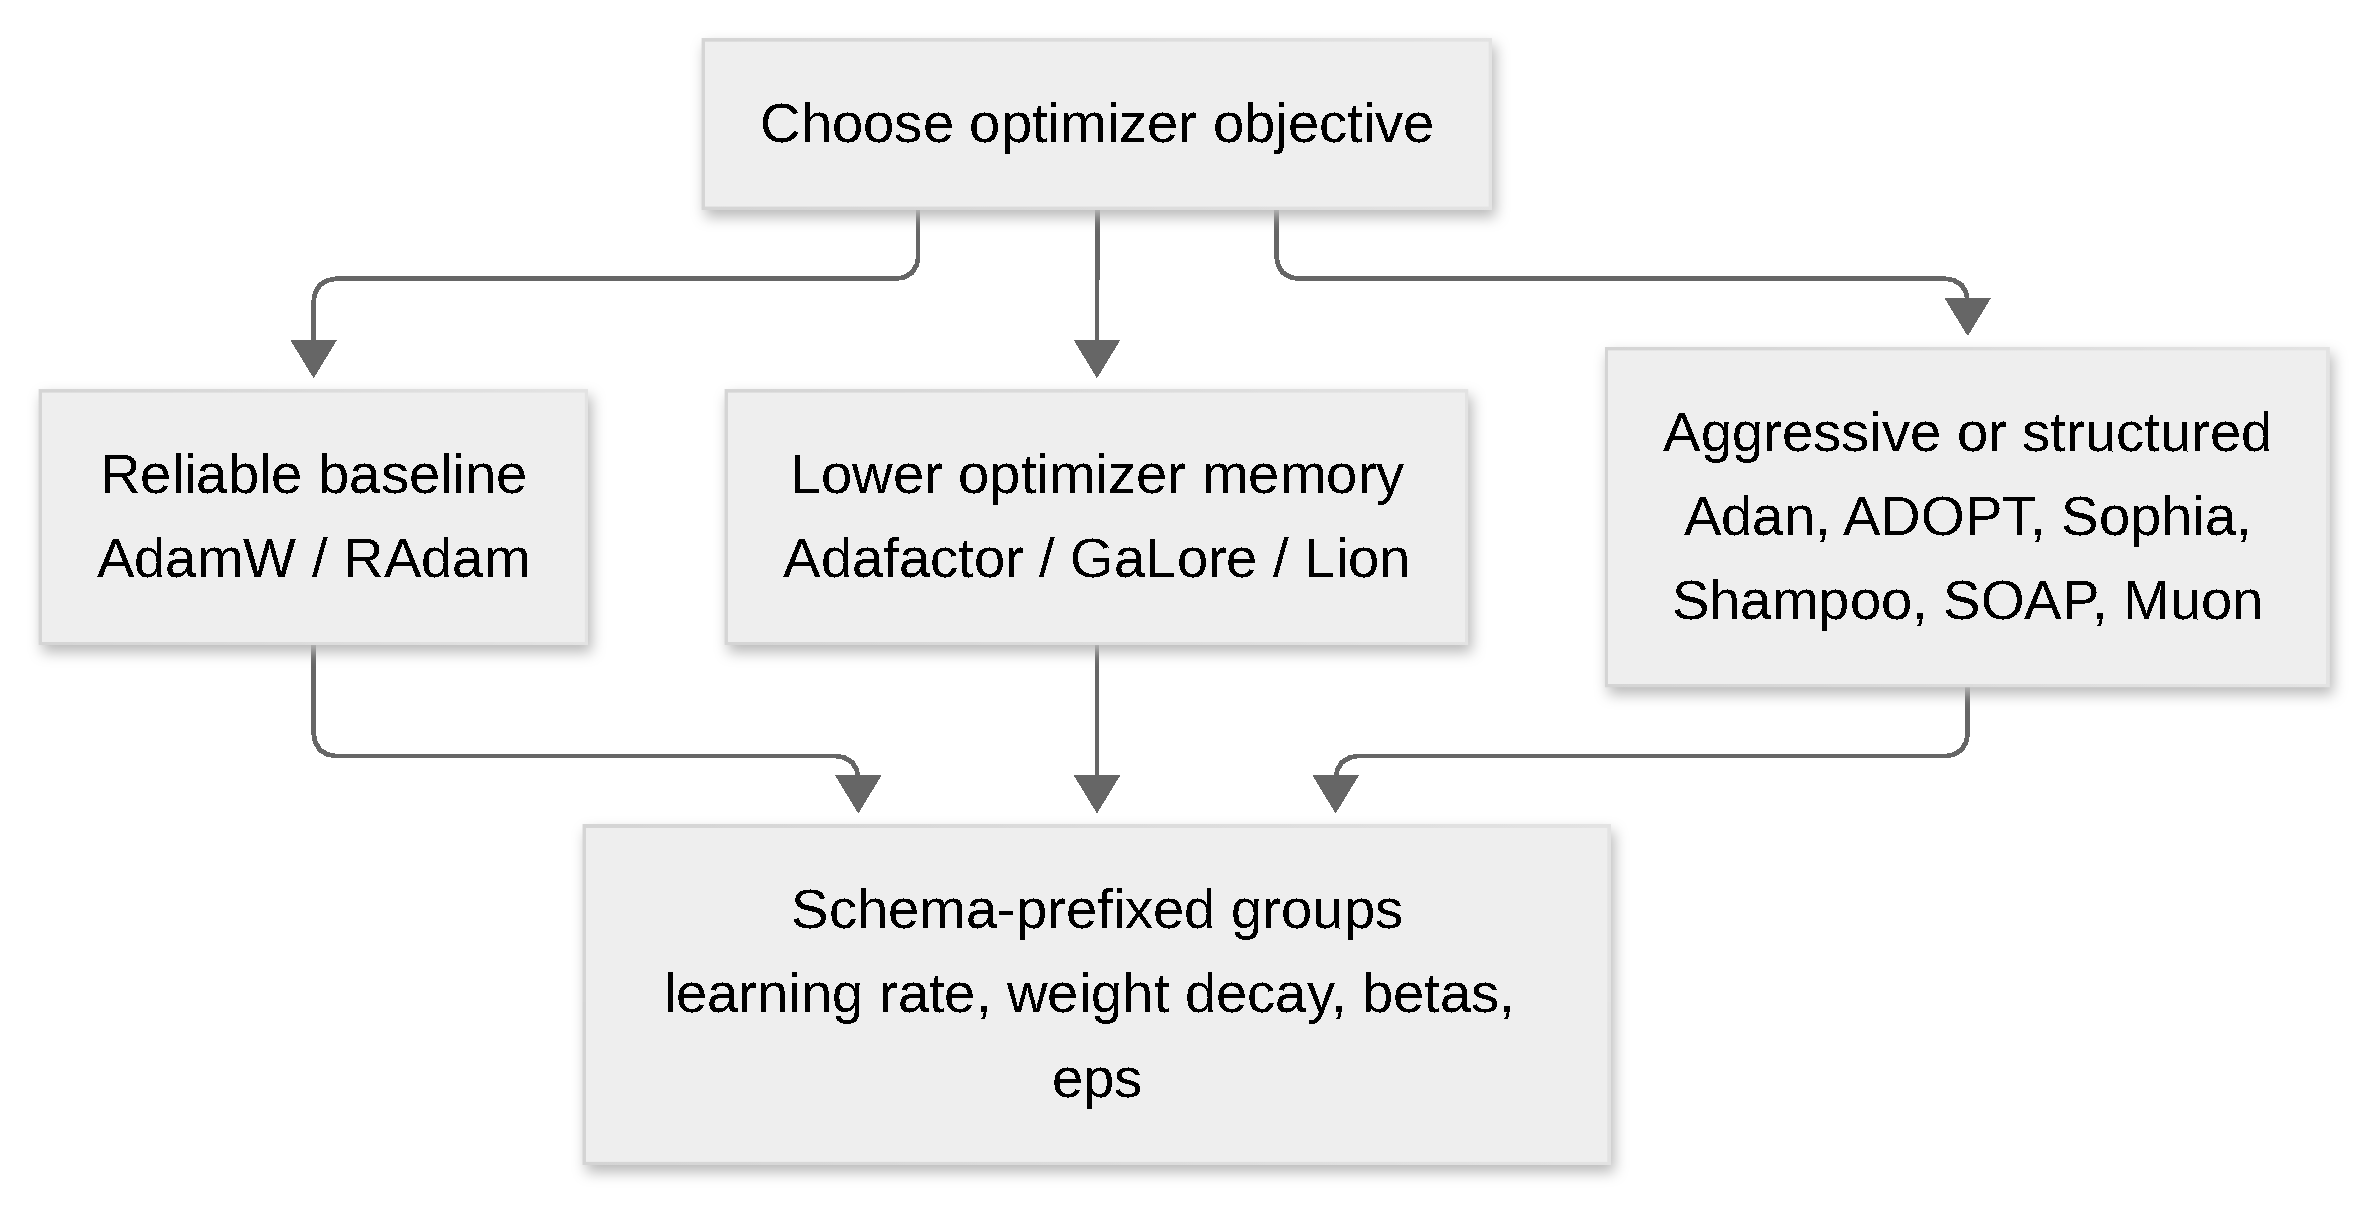
\includegraphics{figures/optimizer-routing.pdf}}
\caption{Optimizer selection in practice: the class determines the update rule, while the schema controls how hyperparameters apply across embeddings, normalization layers, attention blocks, and the remaining parameters.}
\label{fig:optimizer-routing}
\end{figure}
